\documentclass[11pt]{article}

\usepackage[english,italian]{babel}
\usepackage[a4paper, top=2cm, bottom=1.5cm, left=2cm, right=2cm]{geometry}
\usepackage{float}
\usepackage{ltablex}
\usepackage{titling}
\usepackage{blindtext}
\usepackage[utf8]{inputenc}
\usepackage[T1]{fontenc}
\usepackage{xcolor}

\usepackage{natbib}
\usepackage{graphicx}

\usepackage{geometry}
\usepackage[italian]{babel}
\usepackage{tabularx}
\usepackage{longtable}
\usepackage{hyperref}
\usepackage[bottom]{footmisc}
\usepackage{fancyhdr}
\usepackage{titlesec}
\setcounter{secnumdepth}{4}
\usepackage{amsmath, amssymb}
\usepackage{array}
\usepackage{graphicx}
\usepackage{url}
\usepackage{comment}
\usepackage{eurosym}

\title{Valutazione Capitolati}
\author{BugPharma }
\date{14 November 2021}

\begin{document}

\thispagestyle{empty}
	\begin{titlepage}
		\begin{center}
			
\includegraphics[scale = 0.05]{logo_unipd.png}\\
			\large \textbf{Università degli Studi di Padova} \\
			\vfill
			\includegraphics[scale = 0.7]{BugPharma.png}\\
			\large \textbf{Bug Pharma} \\
			\vfill
			\large
			E-mail: 
			\texttt{bugpharma10@gmail.com}
			\vfill
			\Huge \textbf{Valutazione Capitolati 2020/2021}\\
			
			\large
			
			
			\vfill
			
			
			\begin{tabular}{r|l}
				\textbf{Approvazione} &  -\\
				\textbf{Redazione} &  \parbox[t]{5cm}{Lorenzo Piran \\Michele Masetto \\ Sara Nanni}\\
				\textbf{Verifica} &  -\\
				\textbf{Stato} & Redatto \\
				\textbf{Uso} & Esterno
			\end{tabular}
			\vfill
			
		\end{center}
	\end{titlepage}


\maketitle

\tableofcontents
\newpage

\section{Capitolato C5}
    \subsection{Info sul Capitolato} Info sul capitolato
    \begin{itemize}
        \item \textbf{Nome}: Login Warrior, riconoscere e visualizzare i tentativi di accesso non autorizzati
        \item \textbf{Proponente}: Zucchetti S.p.A
        \item \textbf{Committente}: Prof. Tullio Vardanega e Prof. Riccardo Cardin
    \end{itemize}
    \subsection{Descrizione} Descrizione
    
    Lo scopo di questo capitolato, proposto dalla Zucchetti S.p.A, è quello di predisporre e fornire la realizzazione di un'applicazione di visualizzazione dei dati di login a supporto della fase di riconoscimento e distinzione di attività lecite o attività illecite, che possono essere svolte all'interno di un nostro portale.
    
    Per poter quindi fornire ausilio a chiunque voglia per, da un insieme di dati e informazioni contenute in un CSV, risalire a grafici e dataset in grado di predisporre un immediato riscontro visivo della presenza o meno di attività illecite.
    
    \subsection{Studio del Dominio} Studio del Dominio
        \subsubsection{Dominio Applicativo} Dominio Applicativo
        
        Il capitolato si colloca nell'ambito della creazione di grafici e dataset da dati presenti in un CSV. Gli utenti finali sono quindi amministratori di sitemi esposti sul web in cui è possibile autenticarsi per poter usufruire dei servizi cloud messi a disposizione dalla piattaforma web.
        \subsubsection{Dominio Tecnologico} Dominio Tecnologico
        
        Per lo svolgimento del capitolato e per la creazione dell'applicatovo web viene richiesta la conoscenza dell'ambito web, con lo scopo di creare un'interfaccia piacevole e intuitiva:
        \begin{itemize}
            \item \textit{HTML}: per la struttura ed il markup della pagina;
            \item \textit{CSS}: per la presentazione visiva dell'applicativo web;
            \item \textit{JavaScript}: per il comportamento e il trattamento dei dati;
            \item \textit{D3.js}: libreria, Javascript per la manipolazione di documetni basati sui dati;
            \item \textit{Git}: per il versionamento dell'applicativo.
        \end{itemize}
    
    \subsection{Motivazione della scelta} Motivazione della scelta
        \subsubsection{Pro} Pro
        \begin{itemize}
            \item Le tecnologie e la libreria proposta dalla Zucchetti S.p.A sono strumenti molto diffusi e utilizzati nell'ambito della gestione e presentazione dei dati, in più la documentazione è molto diffusa e esaustiva;
            \item La disponibilità mostrata dall'azienda e la voglia di aiutarci e collaborare con noi, mostrandoci quanto effettivamente un nostro risultato positivo possa essere poi effettivamente utilizzato;
            \item Possibilità di ottenre nuove conoscenze molto spendibili poi in futuro nel mondo del lavoro;
            \item Riuscire ad applicare gli insegnamenti avuti dal corso di Tecnologie web.
        \end{itemize}
        \subsubsection{Contro} Contro
        \begin{itemize}
            \item Molti di noi non hanno familiarità con le tecnologie proposte;
            \item Il dover creare un grafico/dataset per permettere ad un occhio umano di individuare al volo un accesso sospetto ed il renderlo più pulito possibile;
            \item confrontarsi con librerie e algoritmi di ML.
        \end{itemize}
    
    \subsection{Conclusioni} Conclusioni
    
    L'ottimo esito della riunione avuta col signor.Gregorio Piccoli e le accortezze prese dall'azienda nonchè l'utilizzo di tecnologie molto stimolanti ci ha portato a scegliere questo capitolato, come capitolato di prima scelta.
    
    \begin{figure}[h!]
        \centering
        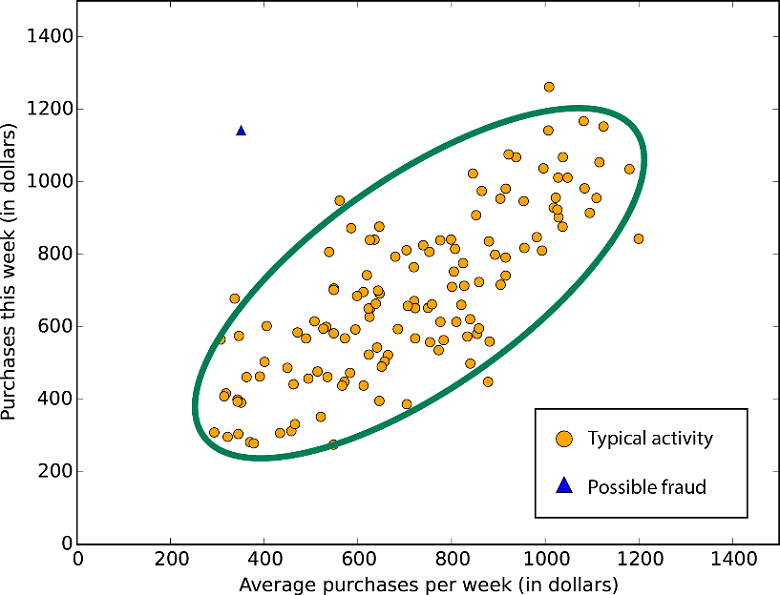
\includegraphics[scale=0.4]{LoginWarrior.png}
        \caption{Grafico accesso utenti}
        \label{zucchetti}
    \end{figure}


\newpage

\section{Capitolato C1}
    \subsection{Info sul Capitolato} Info sul capitolato
    \begin{itemize}
        \item \textbf{Nome}: Bot4Me
        \item \textbf{Proponente}: Imola Informatica
        \item \textbf{Committente}: Prof. Tullio Vardanega e Prof. Riccardo Cardin
    \end{itemize}
    \subsection{Descrizione} Descrizione
    
    Il progetto si focalizza sulla realizzazione di un’applicazione chatbot con lo scopo di aiutare i dipendenti a famigliarizzare con gli strumenti e con il contesto aziendale.
    
    \begin{figure}[h!]
        \centering
        
\includegraphics[scale=0.4]{BotMe.png}
        \caption{Logo Bot4Me}
        \label{Bot4Me}
    \end{figure} 
    
    \subsection{Studio del Dominio} Studio del Dominio
        \subsubsection{Dominio Applicativo} Dominio Applicativo
        
        Il capitolato vuole soddisfare l' esigenza del poter consuntivare le attività giornaliere in un periodo storico dove il Covid-19 ci ha costretto a mutare radicalmente i nostri modi di fare e le nostre abitudini.
        Permettere quindi il tracciamento delle presenze e delle persone, la possibilità quindi poi di creare una nuova riunione e un nuovo ticket sempre secondo la filosofia del tracciamento.
        \subsubsection{Dominio Tecnologico} Dominio Tecnologico
        
        Per lo svolgimento del capitolato e per la creazione dell'applicatovo viene richiesta la conoscenza e la padronanza delle seguenti tecnologie:
        \begin{itemize}
            \item \textit{API  di EMT}: per la registrazione  dell’ingresso e l’inserimento di attività ;
            \item \textit{protocollo MQTT}: per gestire l’apertura del cancello(requisito opzionale);
            \item \textit{API Redmine}: per effettuare l’operazione di inserimento  di un nuovo ticket;
            \item \textit{Git}: per il versionamento dell'applicativo.
        \end{itemize}
    
    \subsubsection{Fattori Critici} Fattori critici
    
    I fattori critici su cui ci siamo soffermati e che ci hanno fatto desistere dall'intraprendere questo capitolato sono:
    \begin{itemize}
            \item molti requisiti obbligatori che richiedono una certa praticità con tecnologie differenti;
            \item difficoltà nel garantire un alto livello di sicurezza senza poter richiedere l’autenticazione per lo strumento in uso;
            \item interpretazione del flusso non solo testuale ma anche vocale.
        \end{itemize}
    \subsection{Conclusioni} Conclusioni
    
    Il dominio applicativo dell'azienda appartiene ad un ambito che ha stimolato pochi di noi, non ci ha spinti verso l'assunzione del capitolato C1, ritenuto da noi molto valido nella sua interezza ma poco incline ai nostri interessi come gruppo.
    
    \newpage

\section{Capitolato C2}
    \subsection{Info sul Capitolato} Info sul capitolato
    \begin{itemize}
        \item \textbf{Nome}: BlockChange - Exchange Platform on BlockChain
        \item \textbf{Proponente}: Sync Lab
        \item \textbf{Committente}: Prof. Tullio Vardanega e Prof. Riccardo Cardin
    \end{itemize}
    \subsection{Descrizione} Descrizione
    
    Viene richiesta la realizzazione di una piattaforma di pagamento digitale che utilizzi come metodo di pagamento un insieme di criptovalute. Lo scopo di tale servizio dovrebbe essere quello di garantire lo scambio di beni tra acquirente e fornitore in maniera sicura e affidabile, in modo tale che nessuna delle due parti sia lesa.
    
    Qui sotto un immagine che riassume il tutto:
    
    \begin{figure}[h!]
        \centering
        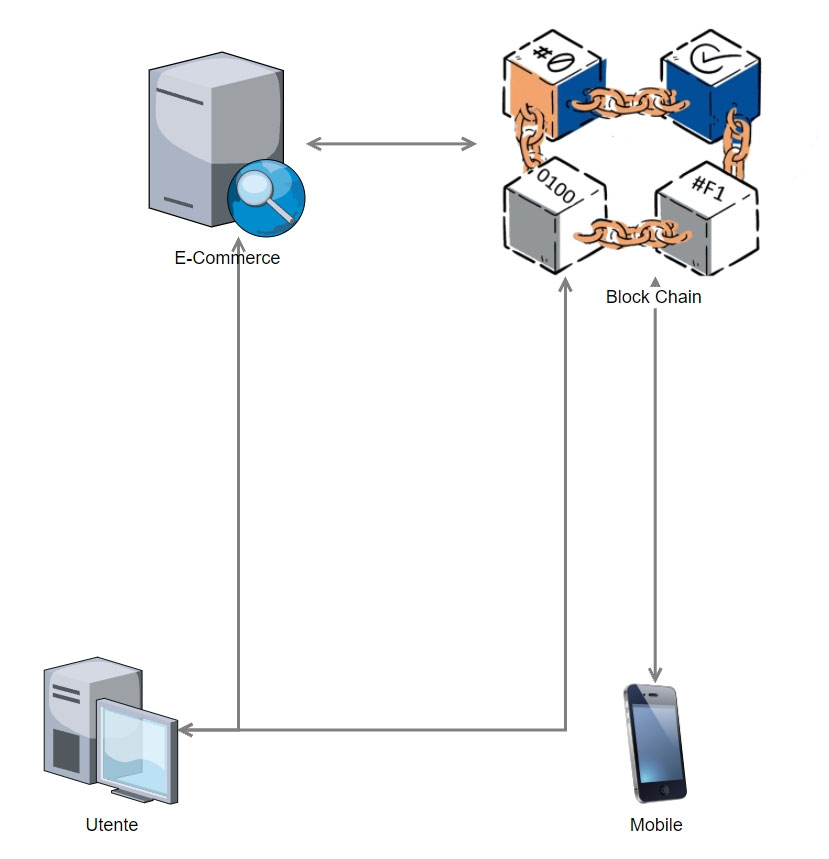
\includegraphics[scale=0.4]{SyncLab.png}
        \caption{Pagamento sicuro e consegna garantita}
        \label{SyncLab}
    \end{figure}
    
    \subsection{Studio del Dominio} Studio del Dominio
        \subsubsection{Dominio Applicativo} Dominio Applicativo
        
        Il capitolato si colloca nell’ambito degli acquisti online, dove da un lato c’è il compratore che desidera acquistare un bene mediante criptovaluta, dall’altro il venditore che vende un prodotto. Il luogo in cui le due parti si incontrano è un e-commerce.
        \subsubsection{Dominio Tecnologico} Dominio Tecnologico
        
        La Proponente preferisce non imporre tecnologie specifiche, ma resta aperta a nuove idee e proposte da parte dei fornitori del capitolato. Tuttavia esprime alcune scelte preferenziali da considerare nello svolgimento del progetto:	
        \begin{itemize}
		    \item  Utilizzo di Blockchain pubblica, come ad esempio Ethereum, con linguaggio \textit{Solidity} da usare per la scrittura degli smart contract; 
			\item Utilizzo di \textit{Java} e \textit{Angular} per lo sviluppo delle parti di Back-end e di Front-end della componente Web Application del sistema; 
			\item Utilizzo di database \textit{PostgreSQL}.
		\end{itemize}
    
    \subsubsection{Fattori Critici} Fattori critici
    I fattori critici su cui ci siamo soffermati ed ci hanno fatto desistere dall'intraprendere questo capitolato sono:
   \begin{itemize}
		\item Scarsa conoscenza da parte del gruppo della Blockchain così come della maggior parte delle tecnologie consigliate;
		\item Risulta difficile gestire il caso in cui un pacco sia smarrito;
		\item Nel caso in cui un pacco sia perso, occorre implementare dei meccanismi di rimborso del venditore da parte di chi si occupa della logistica;
		\item Non è possibile garantire l’anonimato dell’acquirente;
		\item Possono sorgere inconvenienti nel caso di rimborsi dovuti a prodotti malfunzionanti o indesiderati.
	\end{itemize}
    \subsection{Conclusioni} Conclusioni
    
    Inizialmente il gruppo ha preso in considerazione questa proposta. Tuttavia durante gli incontri che si sono tenuti sono emerse delle perplessità riguardanti l’effettiva fattibilità di questo capitolato. L’incontro tenutosi con l’azienda ha risposto solo parzialmente ai dubbi. Si è scelto quindi di escludere questo capitolato.
    
\section{Capitolato C3}
    \subsection{Info sul Capitolato} Info sul capitolato
    \begin{itemize}
        \item \textbf{Nome}: CC4D
        \item \textbf{Proponente}: SanMarco Informatica
        \item \textbf{Committente}: Prof. Tullio Vardanega e Prof. Riccardo Cardin
    \end{itemize}
    \subsection{Descrizione} Descrizione
    
    Il progetto ha lo scopo di creare una web application, sia per mobile che per desktop,che
    permetta all’utente di gestire il controllo statistico dei processi di macchine produttive e 
    le relative caratteristiche da raccogliere in database e visualizzare su grafici.
    
    \subsection{Studio del Dominio} Studio del Dominio
        \subsubsection{Dominio Applicativo} Dominio Applicativo
        
        Il capitolato vuole portare il grupppo attraverso svariati strumenti e tecnologie a  creare un' API per l’immissione della misurazione di una determinata caratteristica, e la creazione di un motore di calcolo che, alla ricezione di una nuova misurazione, si occupi di metterla in relazione con le
        misurazioni precedenti al fine di calcolare se la serie di punti evidenza un processo “fuori controllo”.
        \subsubsection{Dominio Tecnologico} Dominio Tecnologico
        
        Per lo svolgimento del capitolato e per la creazione dell'applicatovo viene richiesta la conoscenza e la padronanzza delle seguenti tecnologie:
        \begin{itemize}
            \item \textit{NodeJS}: libreria JavaScript per la gestione del comportamento dell'applicativo;
            \item \textit{React}: per la parte front-end con js;
            \item \textit{Angular}: per il front-end;
            \item \textit{Git}: per il versionamento dell'applicativo.
        \end{itemize}
    
    \subsubsection{Fattori Critici} Fattori critici
    
    I fattori critici su cui ci siamo soffermati ed ci hanno fatto desistere dall'intraprendere questo capitolato sono:
    \begin{itemize}
            \item Molti temi di ambito differenti che richiedono un buon approfondimento;
            \item Spiegazione del capitolato troppa sintetica; 
            \item Moltitudine di requisiti obbligatori;
            \item Conoscere e dominare bene l'utilizzo di diverse tecnologie;
        \end{itemize}
    \subsection{Conclusioni} Conclusioni
    
    Il dominio applicativo dell'azienda appartiene ad un ambito che ha stimolato pochi di noi, non ci ha spinti verso l'assunzione del capitolato C3, ritenuto da noi molto valido nella sua interezza ma poco incline ai nostri interessi come gruppo.    
    
\newpage
    
\section{Capitolato C4}
    \subsection{Info sul Capitolato} Info sul capitolato
    \begin{itemize}
        \item \textbf{Nome}: Guida Michelin @ social
        \item \textbf{Proponente}: ZERO12
        \item \textbf{Committente}: Prof. Tullio Vardanega e Prof. Riccardo Cardin
    \end{itemize}
    \subsection{Descrizione} Descrizione
    
    L’azienda committente chiede di realizzare una piattaforma che sia una sorta di guida Michelin. Lo scopo dovrebbe essere quindi quello di creare una classifica dei posti di maggiore interesse analizzando i contenuti social prelevati dai social network Instagram e TikTok, e incrociando i risultati ottenuti con le recensioni online. A tale scopo, la piattaforma deve essere in grado di estrapolare dai social informazioni utili a determinare se un posto è giudicato positivamente o negativamente, partendo da ciò che viene condiviso (come commenti testuali, messaggi vocali, immagini, ecc...).
    
    \begin{figure}[h!]
        \centering
        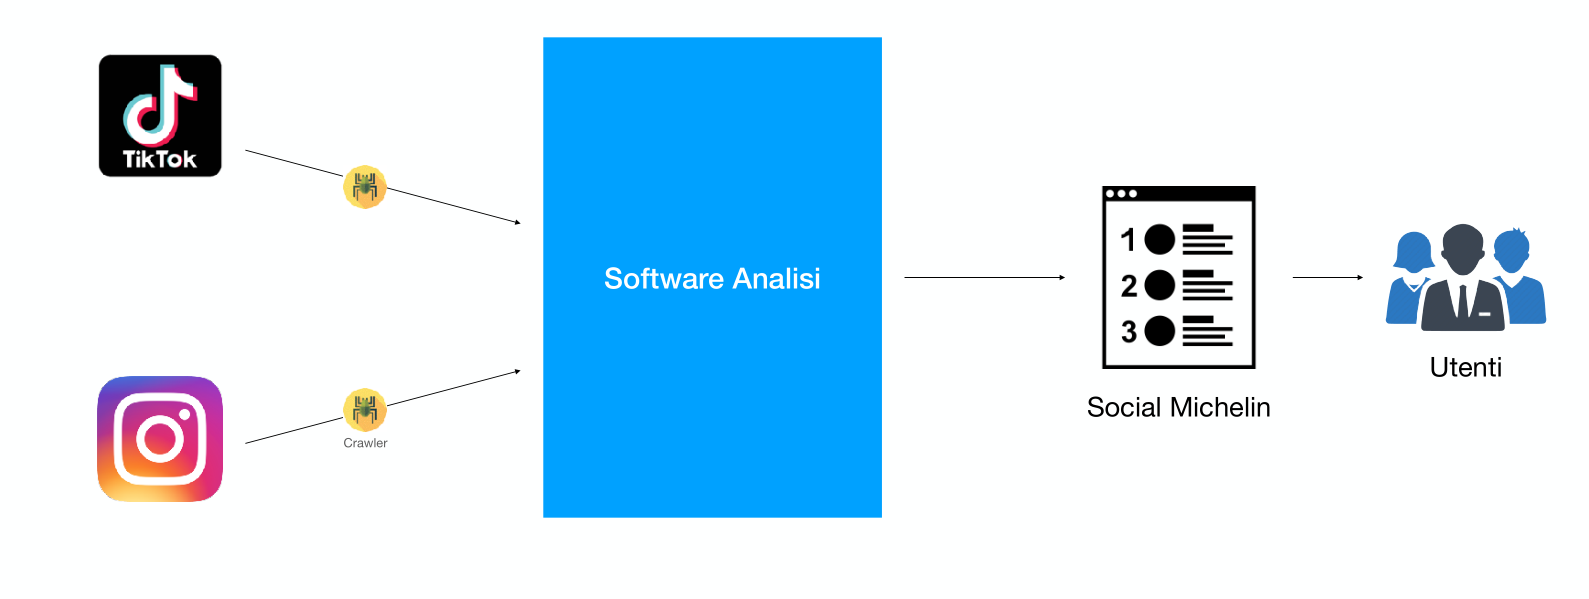
\includegraphics[scale=0.4]{C4.PNG}
        \caption{Ottenimento info dai social}
        \label{GuidaMIchelin}
    \end{figure}
    
    \subsection{Studio del Dominio} Studio del Dominio
        \subsubsection{Dominio Applicativo} Dominio Applicativo
        
        Il capitolato si colloca nell'ambito dei social network.
        Esso vuole offrire ai propri utenti un' esperienza più avvincente possibile utilizzando i contenuti creati pubblicamente dai vari utilizzatori dei social Network, in prevalenza TikTok e Instagram.
        \subsubsection{Dominio Tecnologico} Dominio Tecnologico
        
        Il committente raccomanda di utilizzare la tecnologia di Amazon Web Services ed in particolare i seguenti servizi:
		\begin{itemize}
			\item \textit{AWS Fargate}: servizio Serverless per la gestione a container;
			\item \textit{AWS AppSync}: servizio gestito per lo sviluppo rapido di API GraphQL;
			\item \textit{Neptune}: database a grafo ideale per tracciare per questo tipo di progetti e tracciare efficientemente le relazioni tra i dati.
		\end{itemize}
		I linguaggi di programmazione da utilizzare sono:
		\begin{itemize}
			\item \textit{NodeJS}: linguaggio di programmazione per lo sviluppo di API Restful JSON a supporto dell’applicativo;
			\item \textit{Swift}: linguaggio di programmazione per lo sviluppo di app in ambito iOS/MacOS;
			\item \textit{Kotlin}: linguaggio di programmazione per lo sviluppo di app in ambito Android.
		\end{itemize}
		Inoltre l’architettura deve essere basata a micro-servizi.
    
    \subsubsection{Fattori Critici} Fattori critici
    I fattori critici su cui ci siamo soffermati ed ci hanno fatto desistere dall'intraprendere questo capitolato sono:
    \begin{itemize}
            \item A primo impatto il gruppo si è mostrato scettico sul fatto che, secondo le normative sui dati vigenti di Instagram e TikTok, sia possibile raccogliere i dati degli utenti;
			\item Il capitolato, vista la complessità, risulta essere particolarmente dispendioso in termini di tempo;
			\item Poca esperienza su AWS così come sui linguaggi di programmazione da utilizzare.
        \end{itemize}
    \subsection{Conclusioni} Conclusioni
    
    Il dominio applicativo dell'azienda appartiene ad un ambito che ha stimolato pochi di noi, non ci ha spinti verso l'assunzione del capitolato C4, ritenuto da noi molto valido nella sua interezza ma poco incline ai nostri interessi come gruppo, il capitolato è stato poi scartato anche per via dei molti punti poco chiari.

\newpage

\section{Capitolato C6}
    \subsection{Info sul Capitolato} Info sul capitolato
    \begin{itemize}
        \item \textbf{Nome}: Smart4Energy – A new way in energy monitoring and control
        \item \textbf{Proponente}: Socomec Innovative Power Solutions
        \item \textbf{Committente}: Prof. Tullio Vardanega e Prof. Riccardo Cardin
    \end{itemize}
    \subsection{Descrizione} Descrizione
    
    Il progetto ha lo scopo di cambiare il modo in cui le persone si interfacciano ai dispositivi Socomec e il modo in
    cui viene erogato il servizio di assistenza.
    
    Per poter quindi fornire ausilio per un avanzamento tecnologico ai gurppi di continuità (UPS), per far si che possano essere fruiti ed utilizzati, tramite diverse tecnologie, da differenti device.
    
    
    \subsection{Studio del Dominio} Studio del Dominio
        \subsubsection{Dominio Applicativo} Dominio Applicativo
        
        Il capitolato vuole soddisfare una nuova esigenza nell'ambito dell'UPS derivata dai consumatori.
        Il capitolato vuole proporre all’utente una nuova esperienza d’uso tramite il dispositivo, smartphone o
        tablet, dell’utente stesso.
        In questo modo l’utente sarà naturalmente a suo agio, utilizzando il proprio device per svolgere operazioni riguardanti l'unità di UPS.
        \subsubsection{Dominio Tecnologico} Dominio Tecnologico
        
        Per lo svolgimento del capitolato e per la creazione dell'applicatovo che si interfaccierebbe con l'unità di UPS, viene richiesta la conoscenza dell'ambito mobile, per poter lavorare con apparati mobili che sono dotati, nella quasi totalità, di sistema operativo Android™ o iOS™.
        \begin{itemize}
            \item \textit{Kotlin}: un moderno linguaggio di programmazione lato mobile sviluppato da JetBrains ed in elevata ascesa;
            \item \textit{Java}: dato che i sistemi Android™ sono da sempre stati programmati in Java, per permetterci quindi la più alta configurazione possibile;
            \item \textit{Swift}: per la parte di programmazione relativa ad iOS™;
            \item \textit{Git}: per il versionamento dell'applicativo.
        \end{itemize}
    
    \subsubsection{Fattori Critici} Fattori critici
    I fattori critici su cui ci siamo soffermati ed ci hanno fatto desistere dall'intraprendere questo capitolato sono:
    \begin{itemize}
            \item Molti di noi non hanno familiarità con le tecnologie proposte;
            \item Il fatto che l'azienda proponente abbia come main operativo un campo differente dal nostro; 
            \item Capitolato troppo lungo e dispersivo.
        \end{itemize}
    \subsection{Conclusioni} Conclusioni
    
    Il dominio applicativo dell'azienda appartiene ad un ambito che ha stimolato pochi di noi, non ci ha spinti verso l'assunzione del capitolato C6, ritenuto da noi molto valido nella sua intereza ma poco incline ai nostri interessi come gruppo.
    
    \begin{figure}[h!]
        \centering
        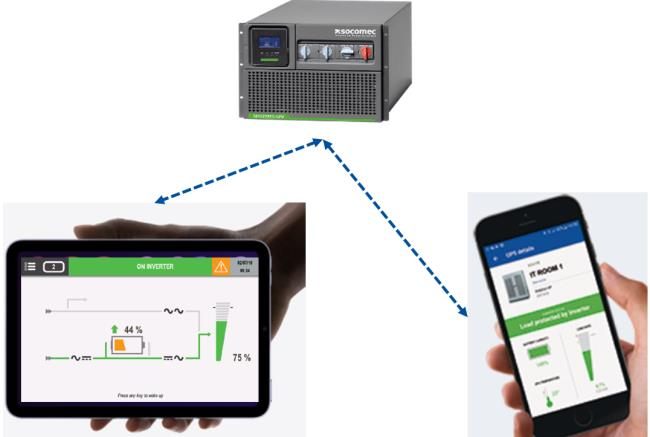
\includegraphics[scale=0.4]{SocomecConnection.png}
        \caption{Connesione dei dispositivi}
        \label{socom}
    \end{figure}

\end{document}
